%%%%%%%%%%%%%%%%%%%%%%%%%%%%%%%%%%%%%%%%%
% Beamer Presentation
% LaTeX Template
% Version 1.0 (10/11/12)
%
% This template has been downloaded from:
% http://www.LaTeXTemplates.com
%
% License:
% CC BY-NC-SA 3.0 (http://creativecommons.org/licenses/by-nc-sa/3.0/)
%
%%%%%%%%%%%%%%%%%%%%%%%%%%%%%%%%%%%%%%%%%

%----------------------------------------------------------------------------------------
%	PACKAGES AND THEMES
%----------------------------------------------------------------------------------------

\documentclass{beamer}
%\usepackage{setspace}
%\doublespacing


\mode<presentation> {

\usetheme{Hannover}

%\usecolortheme{albatross}
%\usecolortheme{beaver}
%\usecolortheme{beetle}
%\usecolortheme{crane}
%\usecolortheme{dolphin}
%\usecolortheme{dove}
%\usecolortheme{fly}
%\usecolortheme{lily}
%\usecolortheme{orchid}
%\usecolortheme{rose}
%\usecolortheme{seagull}
%\usecolortheme{seahorse}
%\usecolortheme{whale}
%\usecolortheme{wolverine}

}

\usepackage{graphicx} % Allows including images
\usepackage{booktabs} % Allows the use of \toprule, \midrule and \bottomrule in tables

%-------------------------------------------------------------------------------
%	TITLE PAGE
%-------------------------------------------------------------------------------


% The short title appears at the bottom of every slide,
% the full title is only on the title page

\title[Path-Energy Optimization]{Quad-Rotor Flight Path Energy Optimization}


\author{Edward Kemper\\Advisor : Niranajan Venkatraman} % Your name


% Your institution as it will appear on the bottom of every slide,
% may be shorthand to save space

\institute[Northern Arizona University]
{
Northern Arizona University \\ % Your institution for the title page
\medskip
\textit{edwardkemper@gmail.com} % Your email address
\medskip
}


\date{April 29, 2014}

\begin{document}


%--------------------------------------------------------------------TITLE SLIDE
\begin{frame}
\titlepage % Print the title page as the first slide
%\begin{centering}

%\end{centering}

\end{frame}


%--------------------------------------------------------------TABLE OF CONTENTS
% Throughout your presentation, if you choose to use
% \section{} and \subsection{} commands, these will
% automatically be printed on this slide as an
% overview of your presentation

\begin{frame}
\frametitle{Overview}
\tableofcontents
\end{frame}


%------------------------------------------------------------------INTRODUCTION
\section{Introduction}

\begin{frame}
\frametitle{Introduction}
\begin{itemize}
\item Tremendous Development
\item Private sector, not just military
\item Autonomy
\item FAA policy for commercial applications (2015)
\item Rapid growth of a multi-billion dollar industry
\end{itemize}
\end{frame}


%--------------------------------------------------------------------MOTIVATION

\begin{frame}
\frametitle{Motivation}
\begin{itemize}
\item Energy management is a pervasive engineering problem
\item Quad-rotors have very high energy demand
\item Multi-rotor systems are entirely thrust driven
\item Instability = Maneuverability = High energy

\end{itemize}
\end{frame}


%--------------------------------------------------------------------PRIOR WORK

\begin{frame}
\frametitle{Prior Work}
\begin{itemize}
\item energy optimization and trajectory planning of fixed wing UAVs
\item quad-rotors
	\begin{itemize}
		\item basic stability
		\item attitude and position control
        \item dynamical model
    \end{itemize}
\item Classical Optimal Control is a long story
\end{itemize}
\end{frame}

%-------------------------------------------------------------PROBLEM STATEMENT

\begin{frame}
\frametitle{Problem Statement}

We wish to find a set of control expressions for a quad-rotor UAV which minimizes the energy expended in flying between two known points in three dimensional space.
\end{frame}

%------------------------------------------------
\begin{frame}
\frametitle{Problem Statement}
\textit{Assumptions:}
\begin{itemize}
\item the flight path that will be optimized is free of obstacles
\item only modeled environmental variables
\item model of the system derived from a Euler-Lagrange formulation
\end{itemize}
\end{frame}

%------------------------------------------------
\begin{frame}
\frametitle{Problem Statement}

\textit{Classical Optimal Control Approach:}

\begin{itemize}
	\item control of the system and the optimization are represented in a single mathematical formulation
	\item Solving the optimal control problem is achieved by solving a boundary value problem
\end{itemize}

\end{frame}



%------------------------------------------------
\begin{frame}
\frametitle{Problem Statement}

\textit{Heuristic approach:}

\begin{itemize}
	\item PD gives attitude control
	\item PID gives position control
	\item this provides a platform for simulation
	\item the optimization procedure evaluates the results of these simulations for optimality as a function of the PID gains used in the position control expressions
\end{itemize}

\end{frame}



%-----------------------------------------------------------------DYNAMIC MODEL
\section{Dynamic Model}


%------------------------------------------------


\begin{frame}
\frametitle{Dynamic Model}

\begin{itemize}
	\item We must understand the mathematical relationships between the control input and the resulting dynamics of the system
	\item Euler-Lagrange formulation
\end{itemize}

\end{frame}




%------------------------------------------------


\begin{frame}
\frametitle{Dynamic Model}


\begin{itemize}
	\item $\psi$ is the yaw angle around the z-axis
	\item $\theta$ is the pitch angle around the y-axis
	\item $\phi$ is the roll angle around the x-axis
\end{itemize}

\begin{figure}
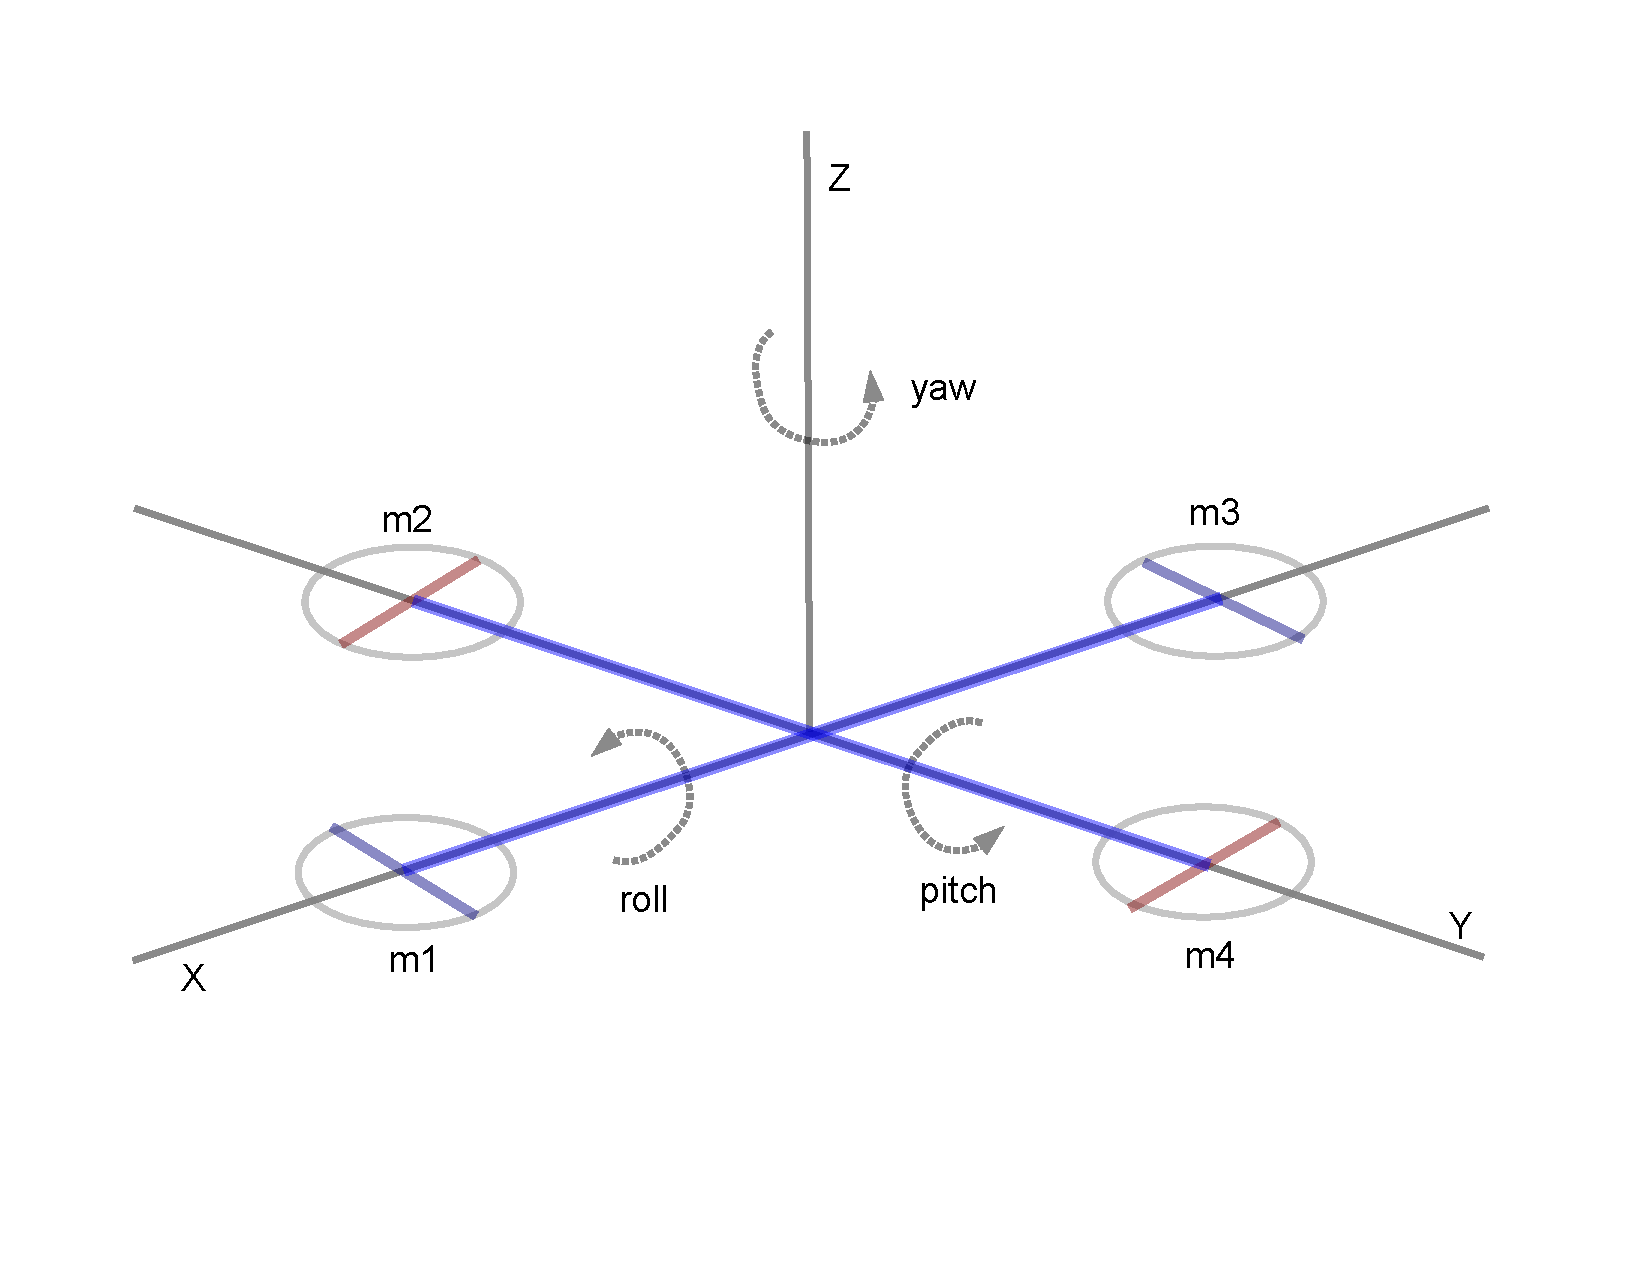
\includegraphics[width=0.8\linewidth]{coords.pdf}
\end{figure}

\end{frame}


%------------------------------------------------

\begin{frame}
\frametitle{Dynamic Model}

The rotor angular velocities are related to the forces they produce by:

\begin{equation}
	f_i = k \omega^2_i
\end{equation}


\end{frame}


%------------------------------------------------

\begin{frame}
\frametitle{Dynamic Model}


In the quad-rotor frame of reference, the motors produce torques on the system.

\begin{equation}
    \label{taub}
    \boldsymbol \tau_B = \left[ \begin{array}{c} \tau_{\phi}\\\tau_{\theta}\\\tau_{\psi}\\ \end{array} \right] = \left[ \begin{array}{c} l s (-\omega_2^2 + \omega_4^2)\\l s (-\omega_1^2 + \omega_3^2)\\ \displaystyle \sum \limits_{i=1}^4 b \omega^2\\\end{array} \right]
\end{equation}

\end{frame}



%------------------------------------------------

\begin{frame}
\frametitle{Dynamic Model}


The combined thrust of the rotors in the direction of the quad-rotor frame $z$ axis is $T_B = [0, 0, T]^T$ where,\\

\begin{equation}
    \label{totalThrust}
    T_B =  \displaystyle \sum \limits_{i=1}^4 f_i
\end{equation}.

\end{frame}


%------------------------------------------------

\begin{frame}
\frametitle{Dynamic Model}

In the inertial frame, the kinetic and potential energy of the system are given by

%translational kinetic energy
\begin{equation}
    T_{\text{trans}}=\frac{1}{2}m\dot{\xi }^T\dot{\xi }
\end{equation}


%rotational kinetic energy
\begin{equation}
    T_{\text{rot}}= \frac{1}{2}\dot{\eta }^T J \dot{\eta }
\end{equation}


% system potential energy
\begin{equation}
    U = m g z.
\end{equation}

The Lagrangian is formed as the difference between kinetic and potential energy.
\end{frame}




%------------------------------------------------

\begin{frame}
\frametitle{Dynamic Model}

\noindent The dynamics of the system are represented by the Euler - Lagrange differential equations of motion.

\begin{equation}
    \frac{d}{\text{dt}} \left( \frac{\delta  L} {\delta \dot{q}}\right) - \frac{\delta  L}{\delta q}=F
\end{equation}

\begin{equation}
 q = [x,y,z,\psi ,\theta ,\phi ]^T = [ \xi , \eta ]^T  .
\end{equation}

\begin{equation}
  \xi  = [x,y,z]^T  \text{ } , \text{ }
  \eta = [\psi ,\theta ,\phi]^T
\end{equation}

\end{frame}



%------------------------------------------------

\begin{frame}
\frametitle{Dynamic Model}

\noindent The linear components of the generalized forces produce the following equations.

\begin{equation}
    \label{linforce}
    f =  R  T_B = m \ddot{ \xi} -  G
\end{equation}


\noindent The angular components are expressed as

\begin{equation}
    \label{eq:angularacc}
    \ddot{\eta} = J^{-1} \big( \tau_b - C(\eta,\dot{\eta}) \dot{\eta} \big)
\end{equation}



\end{frame}



%------------------------------------------------

\begin{frame}
\frametitle{Dynamic Model}
A complete mathematical representation of the quad-rotor is as follows.\\

\begin{equation}
    \label{lineareq}
    \left(
        \begin{array}{c}
           \ddot{x}\\
           \ddot{y}\\
           \ddot{z}\\
        \end{array}
    \right)
    = \left(
       \begin{array}{c}
        0\\
        0\\
        g
      \end{array}
    \right)
    +\frac{T}{m}
     \left(
        \begin{array}{c}
             c_{\psi}S_{\theta}c_{\phi} + s_{\psi}s_{\phi} \\
             s_{\psi}S_{\theta}c_{\phi} - c_{\psi}s_{\phi} \\
             c_{\theta} c_{\phi} \\
        \end{array}
    \right)
\end{equation}

\begin{equation}
    \label{angulareq}
    \left(
        \begin{array}{c}
           \ddot{\phi}\\
           \ddot{\theta}\\
           \ddot{\psi}\\
        \end{array}
    \right) = J^{-1}
    \left[ \left(
        \begin{array}{c}
            l s (-\omega_2^2 + \omega_4^2)\\
            l s (-\omega_1^2 + \omega_3^2)\\
            \sum \limits_{i=1}^4 b \omega_i^2\\
        \end{array}
    \right) -
    C
    \left(
        \begin{array}{c}
           \dot{\phi}\\
           \dot{\theta}\\
           \dot{\psi}\\
        \end{array}
    \right)
    \right]
\end{equation}

\end{frame}




%-----------------------------------------------------CLASSICAL OPTIMAL CONTROL
\section{Classical Optimal Control}

%------------------------------------------------

\begin{frame}
\frametitle{Classical Optimal Control}

\textit{We Define:}
\begin{itemize}
	\item Performance index (Lagrangian) $ L[q(t),u(t),t] = u^T I u $
	\item Constraint equations are the system equations of motion
	\item The Hamiltonian $H = L(q(t),u(t),t) + \lambda(t)^T \big( F(q(t),u(t),t) \big)$
      \item  The full objective function can be written as
\end{itemize}

\begin{equation}
    \mathcal{ J } = \nu^T \Psi ( q(t_f),t_f ) + \int_{t_0}^{t_f}  H(q(t),u(t),t) - \lambda^T \ddot q  dt
\end{equation}


\end{frame}


%------------------------------------------------

\begin{frame}
\frametitle{Classical Optimal Control}

The first variation in J is given by\\

\begin{equation}
    \delta \mathcal{  J  } = \frac{\partial \mathcal{  J  }}{\partial q} \delta q + \frac{\partial \mathcal{  J  }}{\partial \dot q} \delta \dot q   +  \frac{\partial \mathcal{  J  }}{\partial u} \delta u = 0
\end{equation}


\end{frame}



%------------------------------------------------

\begin{frame}
\frametitle{Classical Optimal Control}

By setting the variation of $J$ equal to zero we obtain:

The Co-state equations:

\begin{equation}
\frac{\partial H}{ \partial q } = \ddot \lambda
\end{equation}

\begin{equation}
\ddot \lambda = ( \frac{\partial L}{\partial q}  )^T + ( \frac{\partial F}{\partial q} )^T \lambda
\end{equation}

\end{frame}



%------------------------------------------------

\begin{frame}
\frametitle{Classical Optimal Control}

\textit{and} the Stationarity Conditions:

\begin{equation}
    \frac{\partial H}{\partial u} = 0
\end{equation}

\begin{equation}
    \frac{\partial L}{\partial u} +( \frac{\partial F}{\partial u} )^T \lambda = 0
\end{equation}

\end{frame}



%------------------------------------------------

\begin{frame}
\frametitle{Classical Optimal Control}

\textit{and} Secondary algebraic Co-state conditions

\begin{equation}
    \frac{\partial H}{\partial \dot q} = 0
\end{equation}

\begin{equation}
    (\frac{\partial F}{\partial \dot q})^T \lambda = 0
\end{equation}


\end{frame}



%------------------------------------------------

\begin{frame}
\frametitle{Classical Optimal Control}


\textit{and} Terminal Boundary conditions:

\begin{equation}
    \nu^T \frac{\partial \Psi}{\partial q}|_{t_f} + \dot \lambda(t_f)^T = 0
\end{equation}

\begin{equation}
    \nu^T \frac{\partial \Psi}{\partial \dot q}|_{t_f} - \lambda(t_f)^T = 0
\end{equation}


\textit{and} Initial Co-state conditions

\begin{equation}
    ( \lambda^T \delta \dot q - \dot \lambda^T \delta q )|_{t_0} = 0
\end{equation}

\begin{equation}
    \lambda(t_0)^T \delta \dot q = \dot \lambda(t_0)^T \delta q )
\end{equation}





\end{frame}



%------------------------------------------------

\begin{frame}
\frametitle{Classical Optimal Control}

The optimality conditions form a two-point boundary value problem.

\textit{to obtain a solution:}

\begin{itemize}
	\item the shooting method
	\item finite difference method
\end{itemize}


\end{frame}



%------------------------------------------------

\begin{frame}
\frametitle{The Shooting Method}

\textit{the algorithm:}

\begin{itemize}
\item solving the set of differential equations as an initial value problem

\item measuring the error in the final state of the system compared to the desired final state

\item Advantages
    \begin{itemize}
        \item straightforward iterative quadrature method and error minimization
    \end{itemize}
\item Disadvantages
    \begin{itemize}
        \item does not always converge, subject to the stability of the differential equations in question
    \end{itemize}
\end{itemize}

\end{frame}



%------------------------------------------------

\begin{frame}
\frametitle{The Finite Difference Method}

\begin{itemize}

\item create a system of algebraic equations at each instance in time where the solution is desired
\item derivatives in the differential equations are expressed as finite differences
\item The values of each state and co-state variable are defined as unknowns at each time step
\item thousands of equations and unknowns
\end{itemize}

\begin{itemize}
\item Advantages
    \begin{itemize}
        \item turns the BVP into a system of algebraic equations
        \item easy to solve for linear system
    \end{itemize}
\item Disadvantages
    \begin{itemize}
        \item hard to solve for nonlinear system
        \item does not always converge
    \end{itemize}
\end{itemize}

\end{frame}




%------------------------------------------------

\begin{frame}
\frametitle{Decision Time}

\textit{The BVP takes too long to solve so we must find another way!}\\

A Heuristic Method

\begin{itemize}
\item Control of the system achieved with PID expressions
\item Optimization achieved by appropriately manipulating PID gains in order to change the system behavior
\item Quantify system behavior with performance metrics
\end{itemize}

\end{frame}



%-------------------------------------------------------------------PID CONTROL
\section{PID Control}

%------------------------------------------------

\begin{frame}
\frametitle{PID Control}


\begin{itemize}
\item PID controllers for the x, y, and z directions

\item PD controllers for each of the Euler angles $(\phi,\theta,\psi)$

\item Assume process noise and measurement noise are zero
\end{itemize}

\end{frame}




%------------------------------------------------

\begin{frame}
\frametitle{PID Control}

\textit{PID Control Algorithm}

\begin{enumerate}
\item The position control expressions give 'commanded' linear accelerations
\item The necessary total thrust, pitch, and roll are determined.
\item The commanded torques are given by PD controllers using the commanded yaw, pitch, and roll as angular set points.
\item The motor speeds can then be determined.
\item The system model can be used to obtain the updated state of the system.
\item Repeat.
\end{enumerate}

\end{frame}



%------------------------------------------------

\begin{frame}
\frametitle{Simulation Parameters}

\begin{table}
%\begin{doublespace}
\centering
\begin{tabular}{l l l}
    \hline
    $g = -9.81                  $& $     m / s^2                        $ & acceleration due to gravity\\
    $m = 1                       $& $     kg                                $ & mass\\
    $L = 1                         $& $    m                                 $ & length of quad-rotor arm\\
    $b = 10^{-6}             $& $    N m s^2  / Rad^2       $ & aerodynamic torque coef\\
    $k = 2.45*10^{-6}     $& $   N s^2 / Rad^2            $ & aerodynamic thrust coef\\
    $Ixx = 5.0*10^{-3}    $& $   N m s^2 / Rad            $ & moments of inertia \\
    $Iyy = 5.0*10^{-3}    $& $   ""                                 $ & \\
    $Izz = 10.0*10^{-3}   $& $   ""                                 $ & \\
    \hline
\end{tabular}
\caption[Simulation Parameters]{Simulation Parameters}
%\end{doublespace}
\end{table}

\end{frame}




%------------------------------------------------

\begin{frame}
\frametitle{Arbitrary Sub-optimal Paths}

\begin{figure}[htbp]
    \centering
        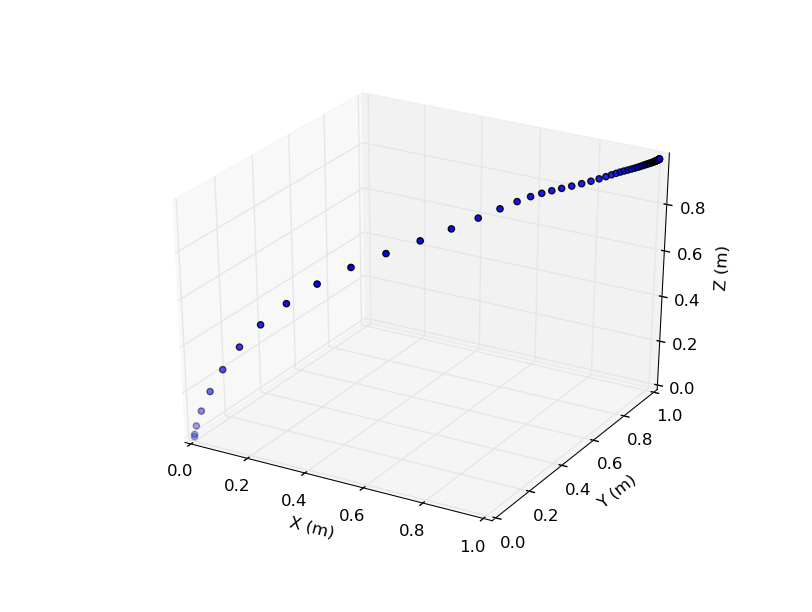
\includegraphics[width=\textwidth]{Figures/typical_run_time_3D_path.png}
        \rule{35em}{0.5pt}
    \caption[typical run 3D path]{A typical run - the 3D path}
    \label{fig:typical run 3D path}
\end{figure}


\end{frame}

%------------------------------------------------

\begin{frame}
\frametitle{Arbitrary Sub-optimal Paths}

\begin{figure}[htbp]
    \centering
        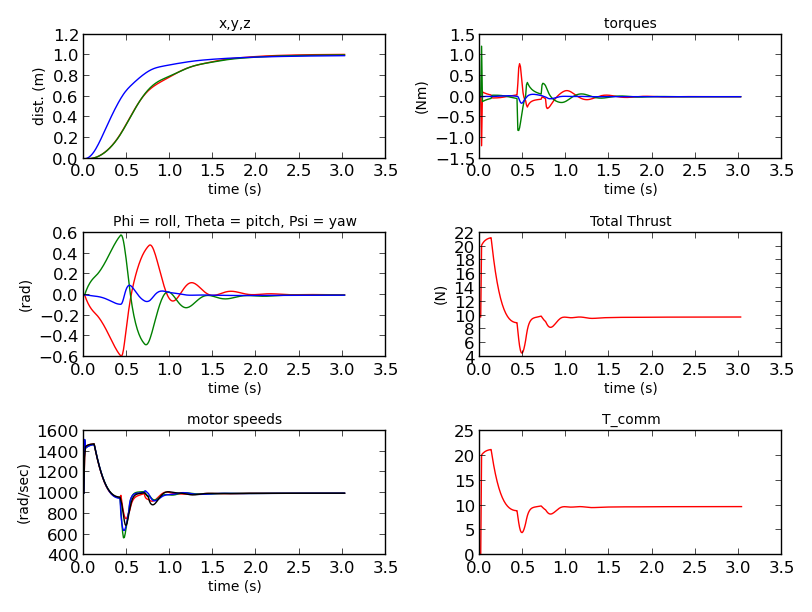
\includegraphics[width=\textwidth]{Figures/typical_run_time_domain.png}
        \rule{35em}{0.5pt}
    \caption[typical run time domain]{A typical run - time domain}
    \label{fig:typical run time domain}
\end{figure}

\end{frame}




%------------------------------------------------

\begin{frame}
\frametitle{Arbitrary Sub-optimal Paths}
\begin{figure}[htbp]
    \centering
        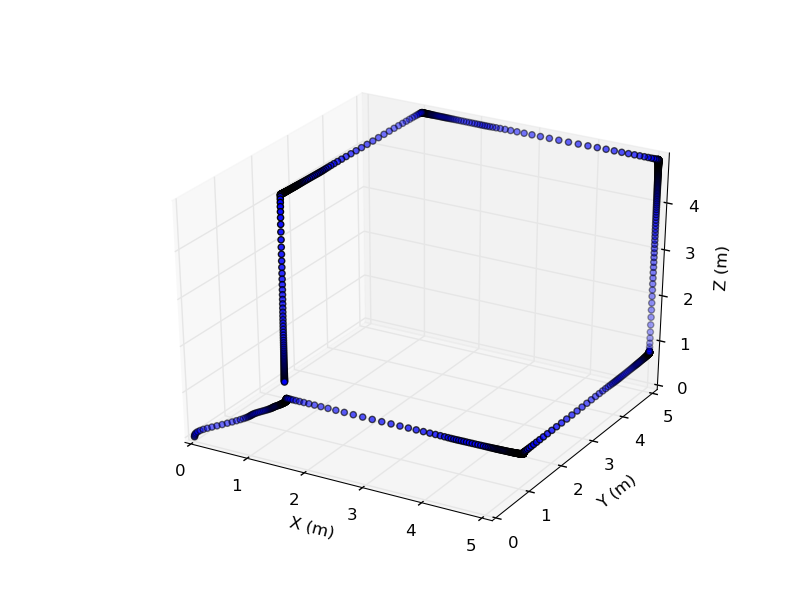
\includegraphics[width=\textwidth]{Figures/CubeEdges3D.png}
        \rule{35em}{0.5pt}
    \caption[Cube Edges]{Tracing some of the edges of a 4m cube - the 3D path}
    \label{fig:Cube Edges 3D}
\end{figure}

\end{frame}



%------------------------------------------------

\begin{frame}
\frametitle{Arbitrary Sub-optimal Paths}
\begin{figure}[htbp]
    \centering
        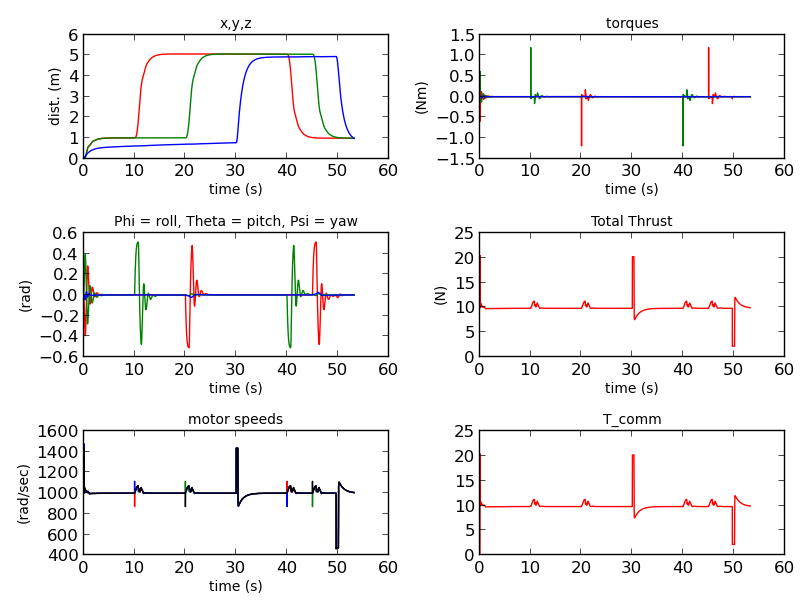
\includegraphics[width=\textwidth]{Figures/CubeEdgesGraphs.png}
        \rule{35em}{0.5pt}
    \caption[Cube Edges]{Tracing some of the edges of a 4m cube - time domain plots}
    \label{fig:Cube Edges Time Domain}
\end{figure}

\end{frame}





%------------------------------------------------

\begin{frame}
\frametitle{Arbitrary Sub-optimal Paths}
\begin{figure}[htbp]
    \centering
        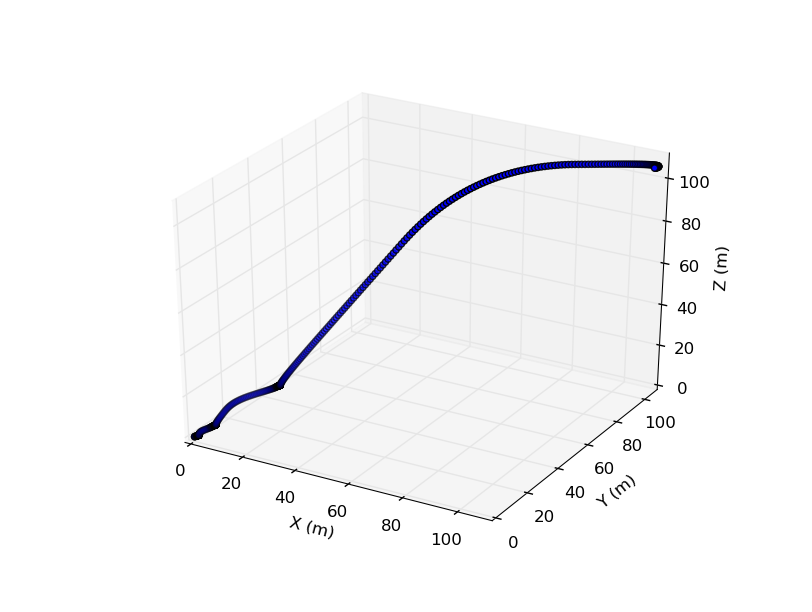
\includegraphics[width=\textwidth]{Figures/largeSetpointDifferencesTest_3d.png}
        \rule{35em}{0.5pt}
    \caption[largeSetpointDifferencesTest3D path]{Testing the control with larger set points - the 3D path}
    \label{fig:largeSetpointDifferencesTest3D path}
\end{figure}

\end{frame}



%------------------------------------------------

\begin{frame}
\frametitle{Arbitrary Sub-optimal Paths}
\begin{figure}[htbp]
    \centering
        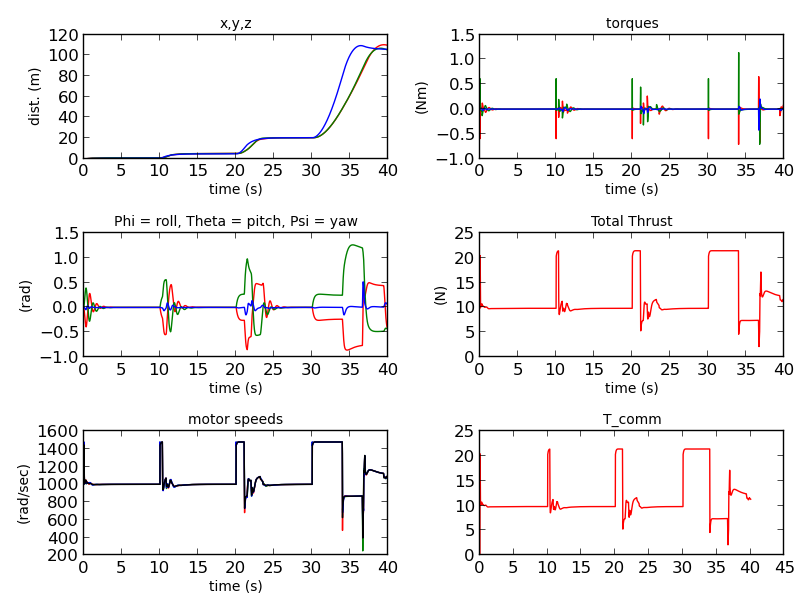
\includegraphics[width=\textwidth]{Figures/largeSetpointDifferencesTest_timedomain.png}
        \rule{35em}{0.5pt}
    \caption[largeSetpointDifferencesTesttimedomain]{Testing the control with larger set points - time domain plots }

\end{figure}

\end{frame}






%---------------------------------------------------------PID GAIN OPTIMIZATION
\section{PID Gain Optimization}

\begin{frame}

\frametitle{ Our Heuristic Optimization Method }

\begin{itemize}
\item We aim to find: $ argmin \big[  \sum_{k,i} \omega_i[k] \text{ } | \text{ } K_p , K_i , K_d  \big]  $
\item $\omega_i[k]$ is the $ith$ rotor speed at the $kth$ time step
\item The variables $K_p$ , $K_i$ and $K_d$ are the vectors of proportional, integral, and derivative gains respectively
\end{itemize}
\end{frame}


%--------------------------------------------------
\begin{frame}

\frametitle{Heuristic Method}

\textit{In reality,there are other important performance criteria}
\begin{itemize}
\item over-shoot of the desired location
\item the time of flight
\item marginal instabilities
\end{itemize}
\end{frame}






%--------------------------------------------------
\begin{frame}
\frametitle{Heuristic Method}

\textit{An Algorithm for Optimization}
\begin{enumerate}
\item Choose a set of proportional and derivative gains for each vector direction (x,y, and,z),
\item Perform a simulation that controls the quad-rotor from an initial vector position to a desired vector position
\item Calculate the sum of the four motor speeds over the duration of the simulation
\item Appropriately change the PID gains such that the sum of the motor speeds decreases
\item Go to step 1. Repeat until the sum of the motor speeds is found to be a minimum.
\end{enumerate}
\end{frame}



%--------------------------------------------------
\begin{frame}

\frametitle{Heuristic Method}

\textit{The relationship between the measured total thrust and PID gains is not well behaved!!}

\begin{itemize}
\item NO steepest descent
\item Needed a deeper understanding of the relationship between PID gains and performance metrics
\item Try brute force approach (?)
\end{itemize}
\end{frame}





%--------------------------------------------------
\begin{frame}

\frametitle{Heuristic Method}

\begin{itemize}
\item Ziegler-Nichols PID tuning method
\item PID gains expressed as a function of $k_u$
\end{itemize}

\vspace{-7mm}

\begin{figure}[htbp]
	\centering
		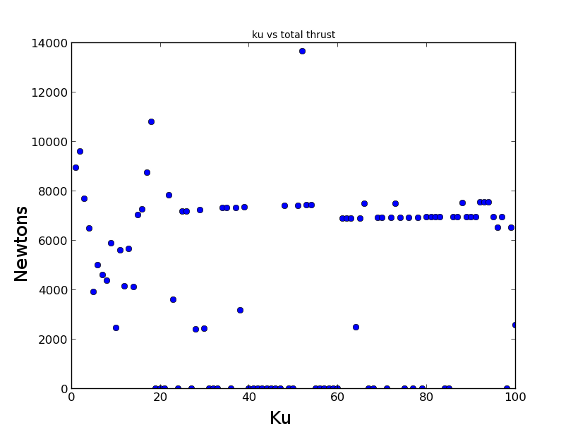
\includegraphics[scale=0.60]{Figures/kuvsthrust.png}
		%\rule{35em}{0.5pt}
	%\caption[ku vs thrust]{The relationship between Ku and the measured total thrust.}
	\label{fig:ku vs thrust}
\end{figure}

\end{frame}


%--------------------------------------------------
\begin{frame}

\frametitle{Brute-Force Results}
{\scriptsize
\begin{table}\label{table:optimalrun}

\centering
\begin{tabular}{l l}
The Optimal Run      \\
\hline
kpx                 & 15 \\
kpy                 & 15 \\
kpz                 & 40 \\
kix                 & 0.8 \\
kiy                 & 0.8 \\
kiz                 & 15 \\
kdx                 & 10 \\
kdy                 & 10 \\
kdz                 & 50 \\
ending iteration    & 987 \\
discrete time step   & 0.01 (s)\\
flight time         & 9.87 (s) \\
cpu runtime         & 11.41 (s)\\
return value        & 1 (great success)\\
initial position    & [0, 0, 1] (m)\\
set point           & [1, 1, 2] (m) \\
total thrust        & 4969.8 (Newton seconds) \\
x crossings         & 3 \\
x overshoot         & 0.0249 (m) \\
y crossings         & 1 \\
y overshoot         & 0.0185 (m)\\
z crossings         & 1 \\
z overshoot         & 0.0992 (m) \\
\end{tabular}

\end{table}
}

\end{frame}





%--------------------------------------------------
\begin{frame}

\frametitle{Brute-Force Results}

\textit{The Optimal Run}
\begin{figure}[htbp]
	\centering
		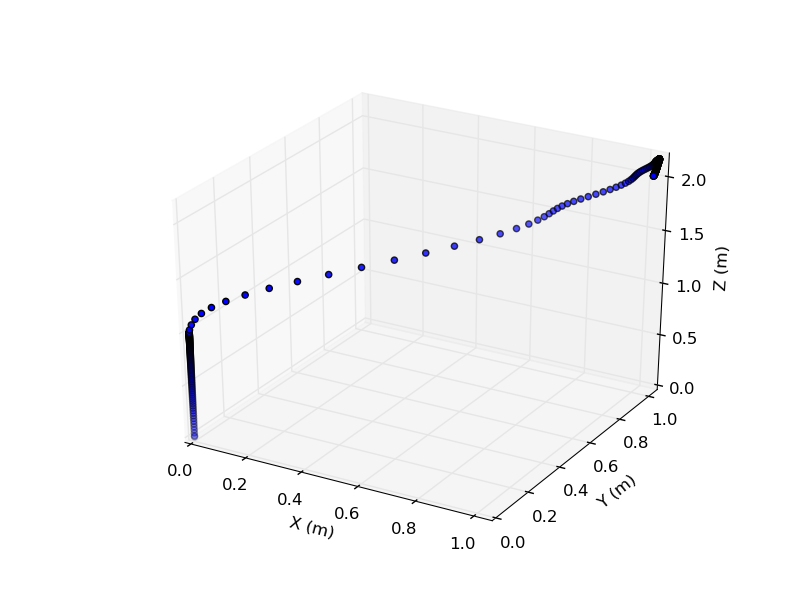
\includegraphics[width=\textwidth]{Figures/optimal_run_3D_path.png}
		\rule{35em}{0.5pt}
	\caption[optimal run 3D path]{The Optimal Run - 3D path}
	\label{fig:optimal run 3D path}
\end{figure}

\end{frame}




\section{Conclusions}%----------------------------------------------CONCLUSIONS


%--------------------------------------------------
\begin{frame}

\frametitle{Conclusions}
\begin{itemize}
\item Classical Optimal Control requires too much computation
\item The Heuristic Method is not viable
\item Brute Force is acceptable

\end{itemize}
\end{frame}


%--------------------------------------------------
\begin{frame}
\frametitle{ Further Work }
\begin{itemize}
\item nonlinear control
\item control / optimization of swarms
\item sensor fusion and state estimation
\end{itemize}
\end{frame}

%--------------------------------------------------------------------REFERENCES


% Beamer does not support BibTeX,
% so references must be inserted manually as below


\begin{frame}

\frametitle{References ({\color{red}DO I NEED REFERENCES IN THE PRESENTATION?})}

\footnotesize{
\begin{thebibliography}{99}
\bibitem[Smith, 2012]{p1} John Smith (2012)
\newblock Title of the publication
\newblock \emph{Journal Name} 12(3), 45 -- 678.
\end{thebibliography}
}
\end{frame}

%------------------------------------------------------------------------------

\begin{frame}
\Huge{\centerline{The End}}
\end{frame}

%------------------------------------------------------------------------------

\end{document}
